\documentclass[11pt]{article}
\usepackage[margin=1in]{geometry}
\usepackage{amsmath, amssymb}
\usepackage{graphicx}
\usepackage{booktabs}
\usepackage{xcolor}
\usepackage{hyperref}
\hypersetup{colorlinks=true, linkcolor=blue, citecolor=blue, urlcolor=blue}

\title{Linear $P(k)$ emulators at $z=0$ for DES halo-model pipelines (v2c)}
\author{J.\ Esteves}
\date{April 2026}

\begin{document}
\maketitle

\section{Introduction}

The halo-model pipeline used in DES cluster analyses
(\texttt{y3\_cluster\_cpp}, \texttt{y1\_mock\_emcee.ini}) requires two
linear matter power spectra: the total matter power spectrum
$P^{\rm mm}(k)$ (includes massive neutrinos) and the CDM+baryon power
spectrum $P^{\rm cb}(k)$, the latter consumed by \texttt{mf\_tinker}
when \texttt{matter\_power\_lin\_version = 2}. A full CAMB evaluation
costs several seconds per cosmology, which dominates the wall time of
any sampling pipeline. We emulate both spectra at $z=0$ with
\textsc{CosmoPower} neural networks and recover the redshift
dependence at inference time through the growth factor,
$P(k, z) = D(z)^2 \, P(k, 0)$, evaluated by the CSL
\texttt{growth\_factor} module. Non-linear quantities ($\sigma(R)$,
$\xi_{\rm NL}(r)$, halo bias $b(M)$) are reconstructed at inference
from the emulated spectra via \texttt{cluster\_toolkit}; only the
truly non-separable non-linear $P(k, z)$ requires a follow-up
emulator, which is discussed in Section~\ref{sec:next}.

The emulators described here (version \texttt{v2c}) are trained on a
combined dataset of $2 \times 10^5$ Latin-Hypercube cosmologies: an
initial broad-prior LHS (\texttt{v2}, $10^5$ samples) augmented with
a Planck-dense LHS ($10^5$ samples) to improve accuracy in the region
where the BAO feature is most sensitive.

\section{Training data and prior}
\label{sec:data}

\paragraph{Priors.} Two Latin-Hypercube samples were generated. The
first (\texttt{v2}) uses broad, flat priors over the six cosmological
parameters. The second (\texttt{v2\_planck}) tightens $\Omega_m$,
$n_s$, and $\log(10^{10} A_s)$ to Planck 2018 $\pm 10\sigma$ and
broadens $\Omega_b$ from v2's overly-tight $[0.05,0.06]$ to a
Planck-consistent range. Table~\ref{tab:priors} summarises both.

\begin{table}[h]
  \centering
  \begin{tabular}{l l l l}
    \toprule
    Parameter & Symbol & v2 range & v2\_planck range ($\pm 10\sigma$) \\
    \midrule
    Hubble           & $h_0$                & [0.40, 1.00]     & [0.40, 1.00] \\
    CDM density      & $\Omega_{\rm cdm}$   & [0.02, 0.65]     & [0.182, 0.338] \\
    Baryon density   & $\Omega_b$           & [0.050, 0.060]   & [0.0376, 0.0608] \\
    Scalar tilt      & $n_s$                & [0.87, 1.07]     & [0.923, 1.007] \\
    Amplitude        & $\ln(10^{10} A_s)$   & [1.64, 4.44]     & [2.904, 3.184] \\
    Neutrino mass    & $\sum m_\nu$ [eV]    & [0.00, 0.20]     & [0.00, 0.20] \\
    \midrule
    (Derived)        & $\Omega_m$           & [0.070, 0.710]   & [0.219, 0.411] \\
    \bottomrule
  \end{tabular}
  \caption{Cosmological priors for the two LHS components of the
  \texttt{v2c} training set. The v2 box is broad and uniform. The
  v2\_planck box is centred on Planck 2018 best fits and tightened to
  $\pm 10\sigma$ on the three parameters that drive the linear $P(k)$
  accuracy ($\Omega_m$, $n_s$, $\ln(10^{10} A_s)$), plus a
  Planck-compatible $\Omega_b$ range derived from
  $\Omega_b h^2 = 0.02208 \pm 0.00052$. Dark energy is fixed to a
  $\Lambda$CDM prescription ($w = -1$, $w_a = 0$, $\Omega_k = 0$)
  with three massive neutrinos in a normal hierarchy and
  $N_{\rm eff} = 3.046$.}
  \label{tab:priors}
\end{table}

To avoid unphysical configurations with $\Omega_b > \Omega_m$ we
sample $\Omega_{\rm cdm}$ directly and set
$\Omega_m = \Omega_{\rm cdm} + \Omega_b$.

\paragraph{CAMB configuration.} Each sample is evaluated at $z=0$
with the CSL CAMB interface.
\texttt{power\_spectra = delta\_tot\ delta\_nonu} returns both
$P^{\rm mm}(k)$ and $P^{\rm cb}(k)$ in a single call. Spectra are
stored on a log-spaced $k$-grid with $k_{\min} = 10^{-4}\,h/$Mpc,
$k_{\max} = 50\,h/$Mpc, and $n_k = 506$ modes, for a row of 512
floats (six parameters $+$ 506 $P(k)$ values) per cosmology per
spectrum.

\paragraph{Dataset.} CAMB returned 99\,939 valid rows from the v2
LHS and 99\,995 from the v2\_planck LHS, for a combined total of
$N_{\rm tot} = 199\,934$ cosmologies after integrity alignment
(linear and CDM+baryon row counts matched per-cosmology; 0.03\% lost
to transient filesystem errors). The combined dataset is shuffled
and split 90/10 into 179\,940 training and 19\,994 test samples, so
the test set covers both broad- and Planck-dense regions.

\section{Emulator architecture and accuracy}
\label{sec:results}

Each emulator is a \textsc{CosmoPower} fully-connected network with
four hidden layers of 512 units and custom sigmoid-based activations,
mapping the six-dimensional parameter vector to $\log_{10} P(k)$
sampled on the 506-mode grid. We train on $\log_{10} P(k)$ because
$P(k)$ spans $\sim 5$ decades over the prior; the network regresses
log-linear features more efficiently. The two emulators share
architecture but are trained independently on $P^{\rm mm}(k)$ and
$P^{\rm cb}(k)$.

Training runs three phases of decreasing learning rate and increasing
batch size: $(10^{-3}, 10^{-4}, 10^{-5})$ and
$(10^3, 5 \times 10^3, 10^4)$ respectively, for
$(400, 800, 1200)$ maximum epochs with a patience of 30 epochs on the
validation loss. An 80/20 internal train/validation split is used
within the 179\,940 training samples.

Accuracy is reported in terms of the fractional residual
\[
  \epsilon(k) \equiv \frac{P_{\rm pred}(k)}{P_{\rm true}(k)} - 1 ,
\]
evaluated on every $(k, \text{cosmology})$ pair in the 19\,994-sample
test set ($\sim 10^7$ predictions per emulator).
Table~\ref{tab:metrics} summarises the test-set performance. The
combined \texttt{v2c} dataset roughly doubles the training volume
over \texttt{v2} and densifies the Planck region, which drives a
$\sim 25$--$35\%$ reduction in every quantile of $|\epsilon|$
relative to the v2-only baseline.

\begin{table}[h]
  \centering
  \begin{tabular}{l c c c c}
    \toprule
    & \multicolumn{2}{c}{$P^{\rm mm}(k)$} & \multicolumn{2}{c}{$P^{\rm cb}(k)$} \\
    \cmidrule(lr){2-3}\cmidrule(lr){4-5}
    Quantity                          & v2      & v2c     & v2      & v2c     \\
    \midrule
    Training samples                  & 89\,945 & 179\,940 & 89\,945 & 179\,940 \\
    Test samples                      & 9\,994  & 19\,994 & 9\,994  & 19\,994 \\
    RMSE $[\log_{10} P(k)]$           & 0.0144  & 0.0104  & 0.0143  & 0.0104  \\
    Median $|\epsilon|$               & 0.089\% & 0.068\% & 0.094\% & 0.076\% \\
    95th percentile $|\epsilon|$       & 0.70\%  & 0.46\%  & 0.75\%  & 0.54\%  \\
    99th percentile $|\epsilon|$       & 2.01\%  & 1.27\%  & 1.95\%  & 1.49\%  \\
    Fraction $|\epsilon| < 1\%$       & 96.9\%  & 98.5\%  & 96.8\%  & 98.1\%  \\
    Fraction $|\epsilon| < 5\%$       & 99.7\%  & 99.9\%  & 99.7\%  & 99.8\%  \\
    \bottomrule
  \end{tabular}
  \caption{Test-set accuracy with $\epsilon = P_{\rm pred}/P_{\rm true} - 1$
  per $(k,\text{cosmology})$, comparing v2 (broad prior only) to
  v2c (broad + Planck-dense). The v2c test set is drawn from the
  shuffled combined dataset; it contains both broad-prior and
  Planck-dense cosmologies and is therefore not directly comparable
  to the v2 test set row-by-row, but it is the honest benchmark of
  the v2c emulator.}
  \label{tab:metrics}
\end{table}

Figure~\ref{fig:err_cdf} shows the cumulative distribution of
$|\epsilon|$ across all test points; both emulators reach 98\% of
predictions below 1\%. Figure~\ref{fig:err_vs_k} shows the
$k$-dependence of the median and 95th percentile; the residual
oscillation near the BAO scale $k \sim 0.1$--$0.3\,h/$Mpc that
limited v2 is strongly suppressed by the Planck-dense samples.
Figure~\ref{fig:examples} compares emulated to true spectra on four
test cosmologies spanning the edges of the $\Omega_m$ and $m_\nu$
priors.

\begin{figure}[h]
  \centering
  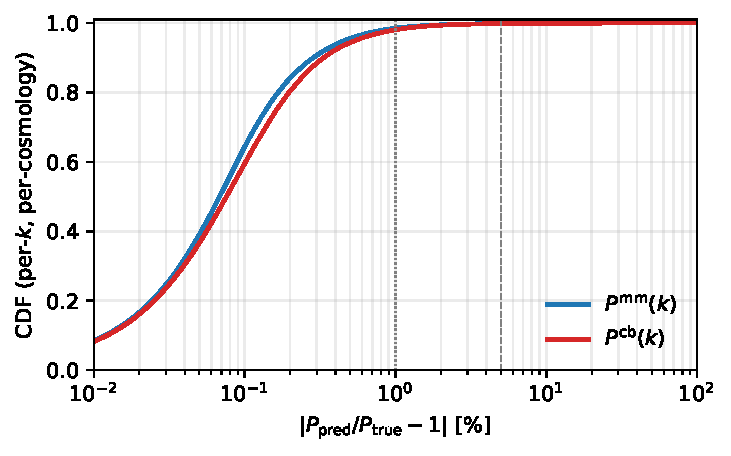
\includegraphics[width=0.55\textwidth]{plots/err_cdf.pdf}
  \caption{Cumulative distribution of $|\epsilon|$ across all
  $19\,994 \times 506$ test points. Dotted line: 1\%; dashed line: 5\%.}
  \label{fig:err_cdf}
\end{figure}

\begin{figure}[h]
  \centering
  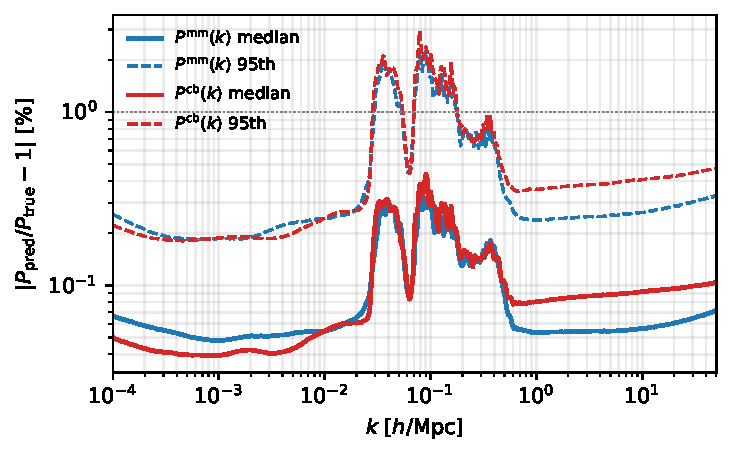
\includegraphics[width=0.55\textwidth]{plots/err_vs_k.pdf}
  \caption{Median (solid) and 95th percentile (dashed) of $|\epsilon|$
  as a function of $k$. Both emulators stay below 1\% on the median
  across the entire $k$-range.}
  \label{fig:err_vs_k}
\end{figure}

\begin{figure}[h]
  \centering
  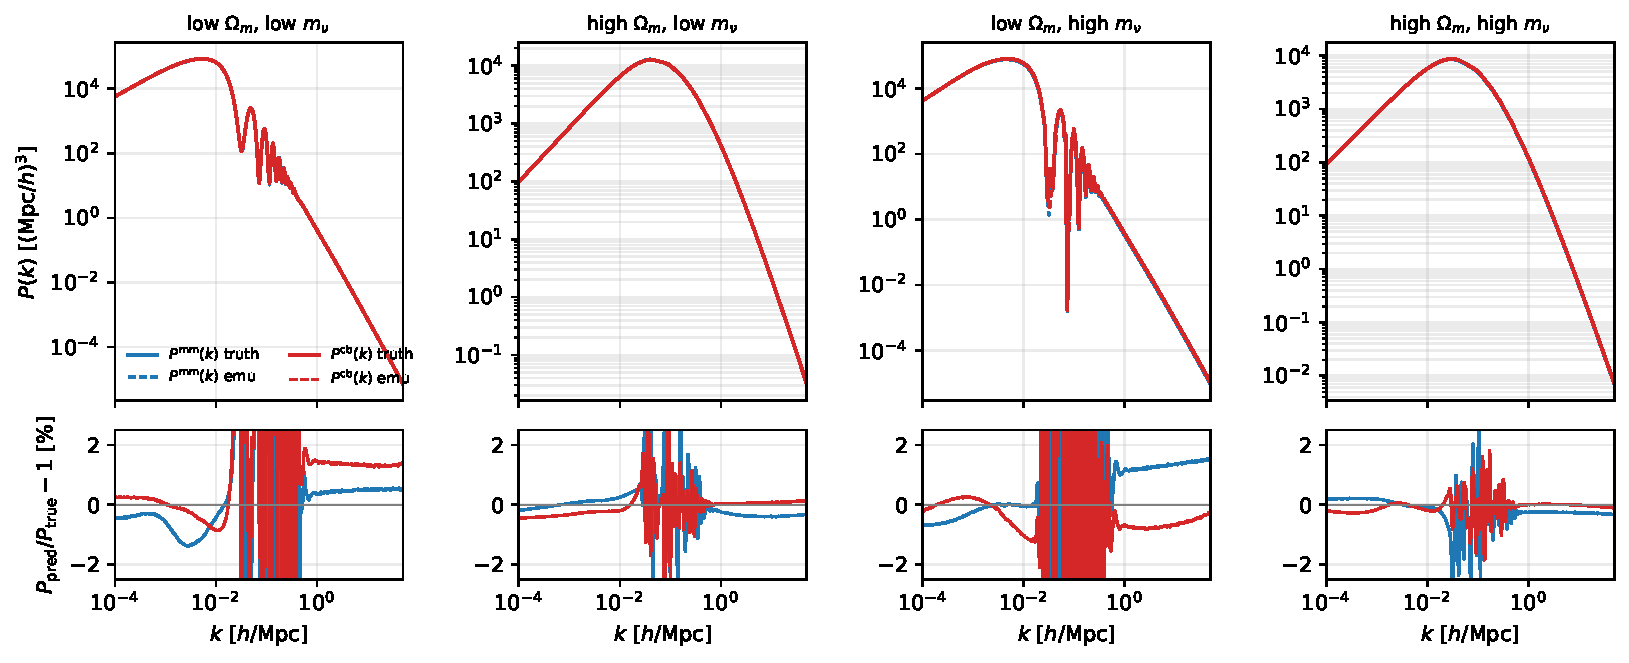
\includegraphics[width=\textwidth]{plots/examples.pdf}
  \caption{Four held-out test cosmologies spanning the corners of the
  $(\Omega_m, m_\nu)$ prior. Top: true (solid) and emulated (dashed)
  $P(k)$ for both spectra. Bottom: fractional residual
  $\epsilon = P_{\rm pred}/P_{\rm true} - 1$ in percent.}
  \label{fig:examples}
\end{figure}

\section{Compute pipeline}
\label{sec:compute}

Both CAMB LHS runs were generated on the Perlmutter CPU partition as
SLURM job arrays. The conda-bundled \texttt{mpi4py} in the shared
cosmosis environment does not link to Cray MPICH, so an MPI launch
fails silently with every rank reporting
$\texttt{Get\_size()} = 1$. We work around this by splitting each
$10^5$-row LHS into 100 slices of 1\,000 samples and running one
serial cosmosis invocation per array task, with each task writing
to a distinct \texttt{slice\{ID\}[planck\_]} file prefix to avoid
concurrent writes on the same inode.

\begin{table}[h]
  \centering
  \begin{tabular}{l l l l l l}
    \toprule
    Step & QoS & Nodes $\times$ CPU/task & Array & Wall/task & Notes \\
    \midrule
    v2 CAMB           & shared     & 1 $\times$ 1 & 0--99, \%20 & $\sim 45$ min    & 100 $\times$ 1\,000 \\
    v2\_planck CAMB   & shared     & 1 $\times$ 1 & 0--99, \%20 & $\sim$60--105 min & 100 $\times$ 1\,000 \\
    Merge $+$ split   & shared     & 1 $\times$ 1 & ---         & $\sim 3$ min     & streaming concat \\
    Clean (.dat $\to$ .npy) & debug & 1 $\times$ 32 & ---        & 30 s            & polars CSV parse \\
    Emulator training & gpu\_debug & 1 $\times$ 32 (1 GPU) & --- & $\sim 7$ min    & A100-80GB, from scratch \\
    \bottomrule
  \end{tabular}
  \caption{SLURM layout of the v2c pipeline. Total CAMB cost dominates
  at $\sim 150$ CPU-hours per LHS ($100 \times 1 \times 1.5$ h
  average for the Planck-dense run). End-to-end wall time from LHS
  generation to trained emulators was $\sim 10$ hours including queue
  waits and the slower Planck-dense wall times.}
  \label{tab:compute}
\end{table}

Table~\ref{tab:compute} lists the per-step SLURM parameters. The
\texttt{shared} qos is ideal for the CAMB arrays because the 0.5-node
cap is not restrictive for a single-core task and its higher
concurrency limit ($\gg \texttt{debug}$'s \texttt{MaxJobsPU=2}) lets
us run 20 tasks in parallel; we throttle with \texttt{\%20} to avoid
dominating the shared scheduler. The Planck-dense run is noticeably
slower per sample than the broad v2 run: CAMB converges its internal
$k$ and $z$ integrations more slowly for cosmologies close to the
physically motivated best-fit point because the halofit and transfer
caches demand tighter tolerances. This is irrelevant for production
--- the emulator is used at inference and completes in milliseconds
--- but it explains why the 2 h wall-time budget was nearly saturated
by the slowest Planck tasks.

\section{Next steps: non-linear $P(k, z)$}
\label{sec:next}

The linear pipeline is separable in $z$, which is why the v2c
emulators are trained at a single redshift. The non-linear pipeline
is not: the halofit prescription introduces a non-trivial
$z$-dependence beyond the linear growth factor, so an emulator of
the non-linear boost
$B(k, z) \equiv P_{\rm nl}(k, z) / P_{\rm lin}(k, z)$ must take $z$
as an explicit input.

\paragraph{Planned setup.} Reuse the six-parameter Planck-dense LHS
from v2c and add $z$ as a seventh input axis, either by broadcasting
each cosmology across an $n_z$-point redshift grid or by drawing an
additional LHS dimension over $z$. The downstream DES pipeline
samples $z \in [0.1, 0.8]$, so a training grid of $n_z = 11$
log-spaced redshifts over $[0, 2]$ (extra margin for $\sigma_R$
integrals and 2-halo integrals out to $z \approx 2$) is sufficient.
The CAMB configuration becomes
\texttt{power\_spectra = delta\_tot\ delta\_nonu} with
\texttt{nonlinear = both}, giving linear and non-linear spectra in a
single call; the boost is $B = P_{\rm nl}/P_{\rm lin}$ computed in
the CosmoSIS save module.

\paragraph{Cost estimate.} With $n_z = 11$, each CAMB call is
$\sim 3\times$ slower than the $z=0$ case because halofit does
internal $k$--$z$ integrations at every output $z$.
100 slices $\times$ 1\,000 samples at $\sim 15$ s per sample gives
$\sim 250$ CPU-hours, plus the same merge/clean/training overhead.
The training network gains a seventh input. Because the boost varies
over a smaller dynamic range ($\sim 0.1$--$10$), the network
typically converges in fewer epochs.

\paragraph{Derived halo-model quantities.} Once both the linear
emulators and the non-linear boost emulator are in place, every
halo-model quantity used by \texttt{y3\_cluster\_cpp} is recoverable
at inference: $\sigma(R, z)$ from the CSL \texttt{sigma\_cpp} on
$P_{\rm lin}(k, z)$; $dn/dM$ from \texttt{mf\_tinker} on
$P^{\rm cb}_{\rm lin}$; $b(M)$ from
\texttt{cluster\_toolkit.peak\_height.nu\_at\_M} on the same; and
$\xi_{\rm NL}(r, z)$ from
\texttt{cluster\_toolkit.xi.xi\_mm\_at\_r} on
$P_{\rm nl} = B \cdot P_{\rm lin}$. No further emulators are required
for the current cluster-cosmology programme. A follow-up direct
emulator of $\sigma(M, z)$ would further reduce the inference-time
bottleneck in \texttt{mf\_tinker}, but this is a second-order
optimisation rather than a necessity.

\paragraph{Validation plan.} The accuracy targets for the non-linear
pipeline flow from the 1\% theoretical error budget on the Tinker
mass function. We will demand the boost satisfy $|\epsilon_B| < 1\%$
at the median and $< 2\%$ at the 95th percentile, and track the
propagated error on $b(M)$ (target: $< 1\%$ at fixed $\nu$) and
$\xi_{\rm NL}(r)$ (target: $< 2\%$ at $r < 100$ Mpc/$h$) on a
held-out set of cosmologies.

\end{document}
